\label{chapter:experiments}
\chapter{Benchmarking and Performance Regression}

By quantifying user experience, we can try to understand it better and improve it. This chapter will focus on experiments that are measuring the performance of the Tribler core, with a particular focus on user experience. Various common operations executed by users in Tribler are identified, discussed and measured.

\section{Experiments environment}
The experiments with the Tribler core are performed on a virtual private server. We tried to keep close to the specifications of a machine that an actual user could be using. The virtual server has 8GB of memory and 1 processor with 4 cores (with a clock speed of 2,5GHz). The used operation system is Ubuntu 15.10.\\\\
If not stated otherwise, the default values of the Tribler configuration file are used. These default values can be found in the `defaults.py` file in the source code directory of Tribler\footnote{https://github.com/Tribler/tribler/blob/devel/Tribler/Core/defaults.py}. All communities, except for \emph{Multichain} and \emph{BarterCast}, are loaded.

\section{Start-up experience}
The very first interaction that users have with Tribler, is the process of starting. During the boot process, many operations are performed:
\begin{itemize}
	\item The connection to the sqlite database is opened. If this database does not exist, it will be created.
	\item Dispersy is started and the enabled communities are loaded.
	\item Various Tribler components are loaded and initialized, including the video streaming server, the REST API, the remote torrent handler and the leveldb store.
\end{itemize}
Booting of the Tribler core happens sequentially and no parallel operations are in place to speed up the process.\\\\
To measure the average start-up time, Tribler is started 30 times. In half of the runs, Tribler is started for the first time, with no prior existing state directory. In the other half of the runs, a database with a little over 100.000 torrents is used. This database is the result of running Tribler idle for several hours, after subscribing to many popular channels. Moreover, a filled Dispersy database is used for the second half of the runs. In both scenarios, there are no downloads running. The experiment starts when the \emph{start} method of the \emph{Session} object is called and ends when the notification that Tribler has started, is observed. The results are displayed in Figure \ref{fig:startup_experiment}.\\\\
It is clear that that size of the database has impact on the time for Tribler to completely boot. However, this impact is relatively minor since Tribler still starts within a second. In both plots, we see some outliers. Further analysis learns us that these outliers are caused by the loading process of the communities.

\begin{figure}[!h]
	\centering
	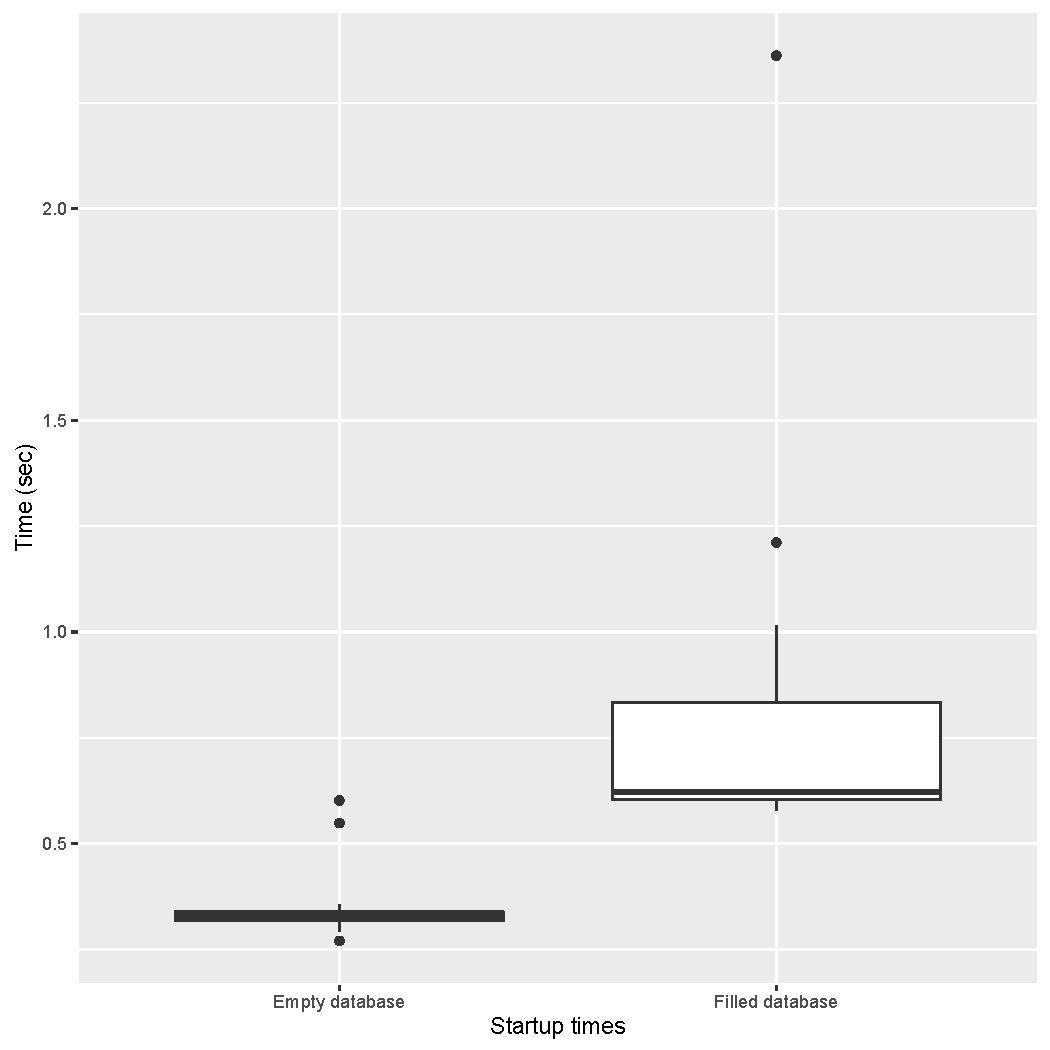
\includegraphics[width=0.6\columnwidth]{images/experiments/startup}
	\caption{Test.}
	\label{fig:startup_experiment}
\end{figure}

\section{Content Search}
We wish to serve relevant information to users as fast as possible. To help users search for relevant content, a remote keyword search has been implemented. Matching search results can either be torrents or channels. Channel results are fetched by a query in the \emph{AllChannel} community whereas torrent results are retrieved by a query in the \emph{search} community.\\\\
To verify the speed of the remote search, various experiments are conducted. We are using a list of 100 terms that users might be searching for. Each query is executed when there are enough peers in the respective communities.

\section{Local keyword search}
...

\section{Video streaming}
...

\section{Content discovery}
...

\section{Channel subscription}
...

\section{Fetching metainfo of torrents}
...

\section{Performance on low-end devices}
...